

Fuzz testing is a popular technique for automatic software vulnerability detection, 
however it suffers from the low efficiency bottleneck when being applied to real-world software. 
This is because modern software have ({\color{red}{has}}) complex input formats, ({\color{red}{e.g., }}) 
 which determine ({\color{red}{such}}) that most of the test cases generated 
 by fuzz testing will be discarded on the shallow surface of programs. 
 Coverage based fuzz testing improves the performance of traditional fuzz testing 
 by collecting all test cases that contribute to coverage into a seed file queue, 
 and all the test cases in this queue will be picked up as the template file for a new cycle of mutation.
 By utilizing such genetic method 
 ({\color{red}{what is the genetic method? If this is necessary to mention, explain how it works on seed files.}}), 
 the fuzzer can quickly touch more new paths and find more bugs 
 than traditional fuzz testing. 
 However, treating the software as a gray box determines it still cannot trigger the bugs 
 that deeply nested in complex code areas.  

Hybrid testing method improves the efficiency of fuzzing testing 
 by employing the advantages of symbolic execution.
 {\color{red}{Another technique to improve the efficiency of fuzzing testing is Hybrid testing.
 In hybrid testing, symbolic execution is exploited to cover the corner cases 
 that are difficult for classical fuzzers to cover. }}
 This is because symbolic execution can easily cover the corner cases 
 that are difficult for fuzzer to cover. 
 Meanwhile, symbolic execution can also benefit from the seed files in the queue from fuzzer 
 to quickly reach more wider code areas. 
 Driller, which is built on top of Angr symbolic execution engine \cite{} and AFL fuzzing engine \cite{}, 
 has attempted to leverage symbolic execution to solve the branches guarded 
 by complex path conditions to avoid the saturation of fuzzer \cite{stephens2016driller}. 
 And its performance in the CGC challenge \cite{online:CGC} demonstrates the potential of this hybrid testing approach.

However, the performance gain from symbolic execution in hybrid testing is still affected ({\color{red}{limited}}) 
 by some program structures(e.g., symbolic pointers and loops). 
 Such structures will quickly generate many states that cannot trigger new behaviors 
 but raise the intrinsic \textit{path explosion} problem of symbolic execution.
 Meanwhile {\color{red}{Moreover}}, by leveraging symbolic execution, 
 the seed queue (including the initial seeds) of the fuzzer will quickly reach a large number for modern software. 
 So when given the testing time budget, the seed queue should be rearranged to make sure 
 that the test case that has greater probability to ({\color{red}{with greater probability of triggering}}) 
 trigger new paths will be tested with high priority.  

In this paper, we introduced ({\color{red}{propose two advanced techniques}}) 
 two improvements to ease the \textit{path explosion} problem 
 raised from the symbolic pointers and loops when using symbolic execution to assist coverage based fuzz testing. 
 Symbolic pointers are lazily concretized to cover more branches and limit the number of states. 
 Based on the loop bucket mechanism of AFL \cite{}, 
 we introduced an optimization to avoid generating too many states when handing symbolic loops. 
 To address the large size of seed queue, 
 we proposed a distance based seed prioritization method for fuzz testing to speed up the path discovery. 
 Each test case in seed queue is enhanced with an weight value 
 which is obtained from the execution runtime information which includes path coverage and memory coverage.
 Our method prioritizes the seed queue according to this weight value and 
 then selects the seed file with the greatest weight value for next mutation cycle.
 And we also designed and implemented the prototype which is built on top of our method. 
 Figure~\ref{Framework} shows the high level framework of our prototype.
 Our main contributions consist of two main components, namely \emph{Symbolic Path Finder} and \emph{Seacher}. 
 The \emph{Symbolic Path Finder} is leveraged to help the fuzzer to dive into deeper code areas 
 that ({\color{red}{are}}) guarded by complex path constraints. 
 Easing the \textit{path explosion} problem ({\color{red}{Technique to handle the path explosion problme}}) 
 raised by symbolic pointers and loops 
 is implemented inside of \emph{Symbolic Path Finder}. 
 The \emph{Searcher} is designed to select the most promising seed file 
 from the seed queue based on the distance measurement. 
 By doing this, the fuzzer will touch more virgin code areas as soon as possible in a time budget. 
 Furthermore, some additional evaluations ({\color{red}{do not say additional.}}) 
 on different benchmarks are performed to demonstrate the ability ({\color{red}{capability}}) of our methods.

\begin{figure}
\begin{center}
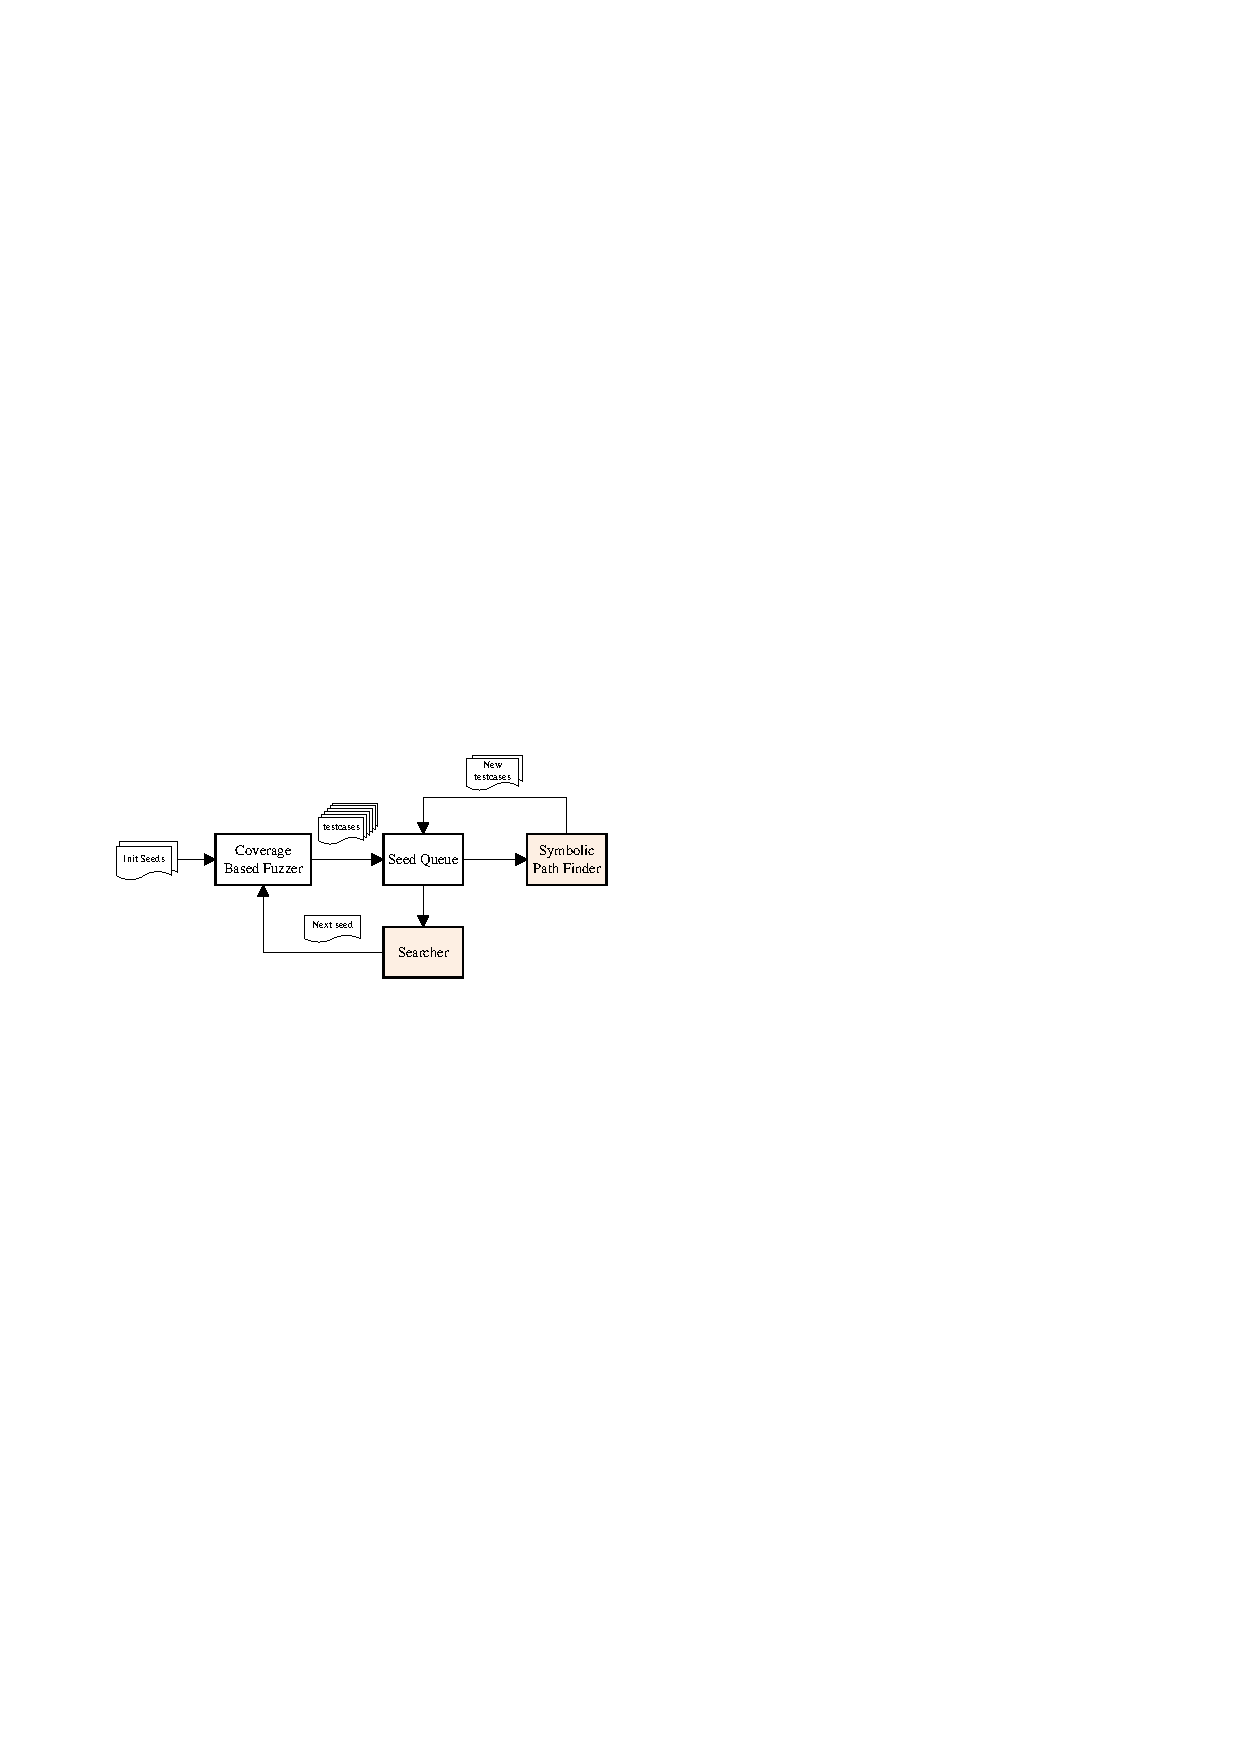
\includegraphics[width=0.7\textwidth]{figures/framework.pdf} 
\caption{High Level Framework.}\label{Framework}
\end{center}
\end{figure}


{\color{red}{This introduction is better now. Still much work should be done on the contribution part.
 Let's proceed this way. 
 Remove the duplications first. What you present above overlaps the following summary.
 Try to present a general workflow of your method, and your contributions using the figure you have.
 You are explaining the boxes of the figure.
 It would be better to state your contributions with the help of the figure. }}


In summary, this paper makes the following contributions.
\begin{itemize}
\item A novel \emph{lazily concretization} method for symbolic pointers is 
 proposed to cover new branches by avoid generating more states, 
 we also present an optimization namely \emph{symbolic loop bucket} 
 for symbolic loops to ease the \emph{path explosion} problem when using symbolic execution to assist fuzz testing.
 ({\color{red}{What is lazily concretization? concretation of what? There are two sentences, comma is not misued.}})

\item A \emph{distance based seed selection} method is proposed to select the most promising seed 
 in the queue to improve path discovery when testing time is limited. 

\item We implemented the prototype based on our method, 
 and the evaluation results on several benchmarks demonstrate the ability of our method for different viewpoints.
\end{itemize}


The rest of this paper is organized as follows. Section~\ref{sec:ease PE} presents the technique details of how we deal with \textit{path explosion} raised from symbolic pointers and loops. The distance based seed selection method is discussed in Section~\ref{sec:seed selection}. Section~\ref{sec:evaluate} describes the implementation of our prototype and the evaluation results. Section~\ref{sec:discussion} discusses the limitations of our work and possible counter measures. Section~\ref{sec:related} reviews the related work, and Section~\ref{sec:conclusion} concludes this paper.
